% Domain grid visualisations (DST grid + interior degrees of freedom).
%
% Requires in the preamble:
%   \usepackage{graphicx}
%   \usepackage{subfig}
%
% The figures live next to this file, in results-paper/grid-visualisation/.
% If you \input this snippet from elsewhere, point graphicx at that folder, e.g.
%   \graphicspath{{results-paper/grid-visualisation/}}
% and drop the leading path from the \includegraphics arguments below.
%
% Excluded on purpose: the "square" and "small_rectangle" domains.

\begin{figure}[htbp]
  \centering
  \subfloat[Rectangle, length $2\pi$, height $\pi$, $M = 49$, DOF $= 1176$.]{%
    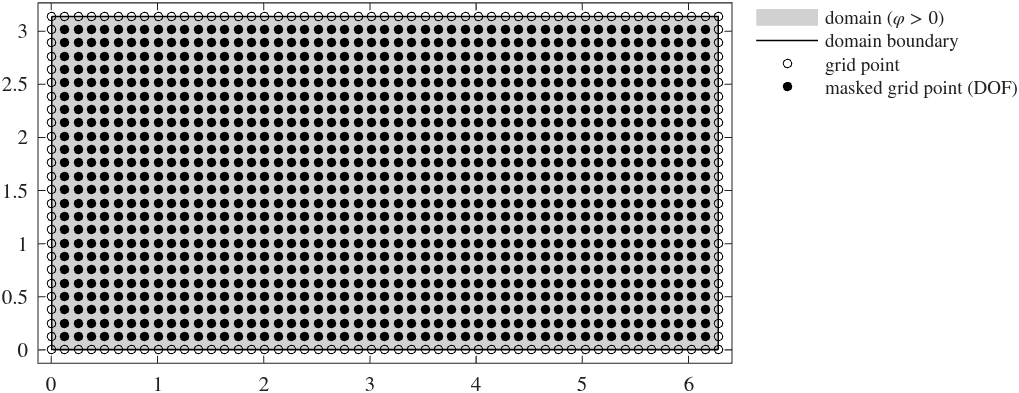
\includegraphics[width=0.4\textwidth]{rectangle_grid_M49_dofs1176}}
  \qquad
  \subfloat[Ellipse (semi-axes $2 \times 1$) minus the fourth quadrant, $M = 47$, DOF $= 649$.]{%
    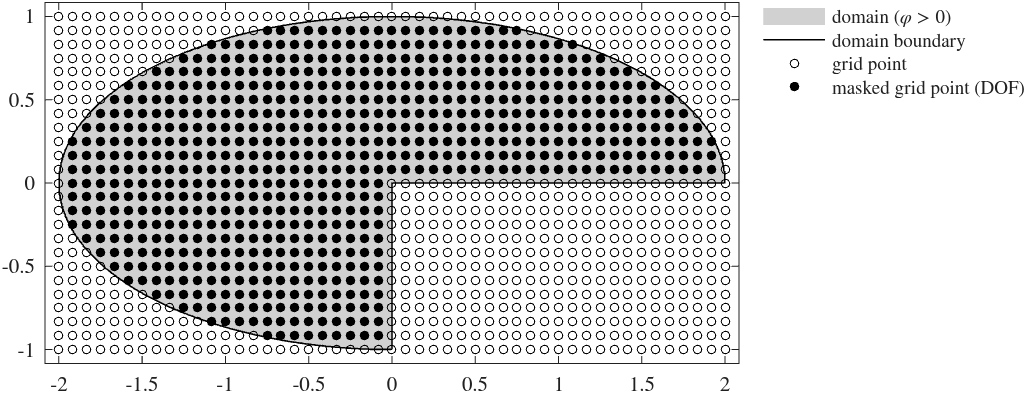
\includegraphics[width=0.4\textwidth]{ellipse_minus_quadrant_grid_M47_dofs649}}
  \\
  \subfloat[Right isosceles triangle, legs length~$\pi$, $M = 50$, DOF $= 1225$.]{%
    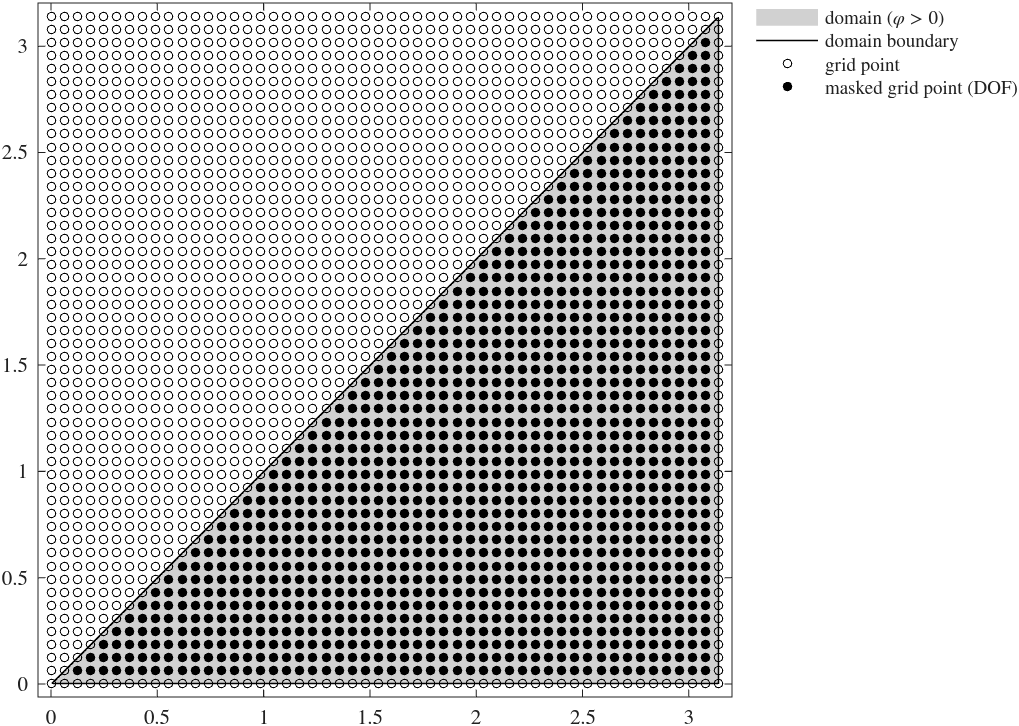
\includegraphics[width=0.4\textwidth]{isosceles_triangle_grid_M50_dofs1225}}
  \qquad
  \subfloat[L-shaped domain, square domain $2 \times 2$ minus a $1 \times 1$ top right corner, $M = 49$, DOF $= 1776$.]{%
    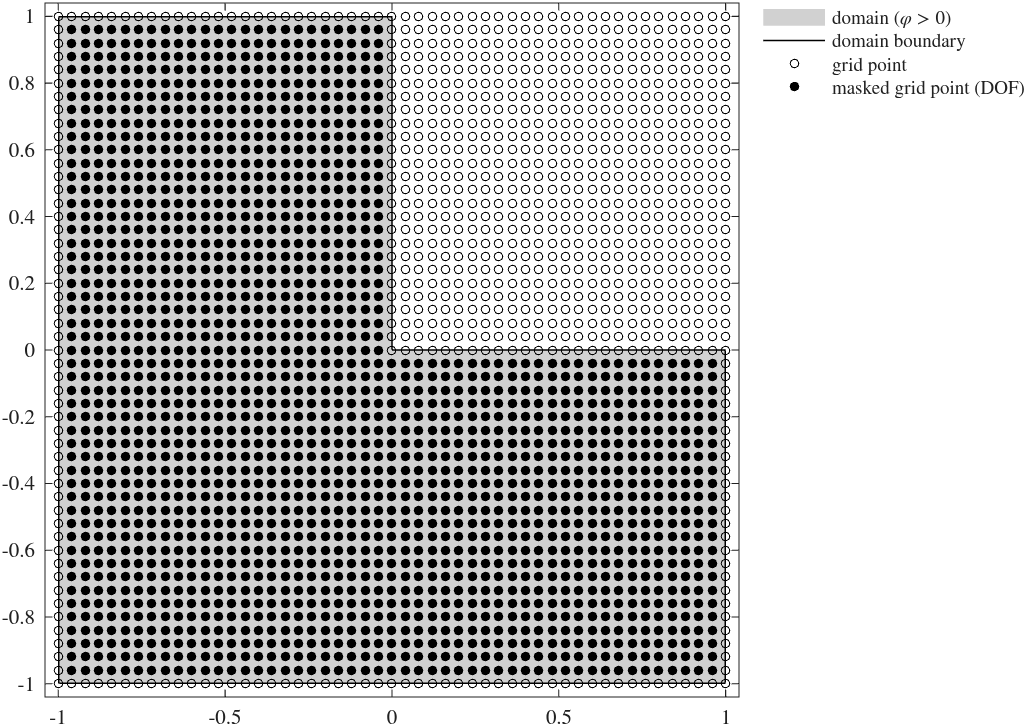
\includegraphics[width=0.4\textwidth]{L_shaped_grid_M49_dofs1776}}
  \\
  \subfloat[GWW drum 1, unit building blocks, $M = 50$, DOF $= 936$.]{%
    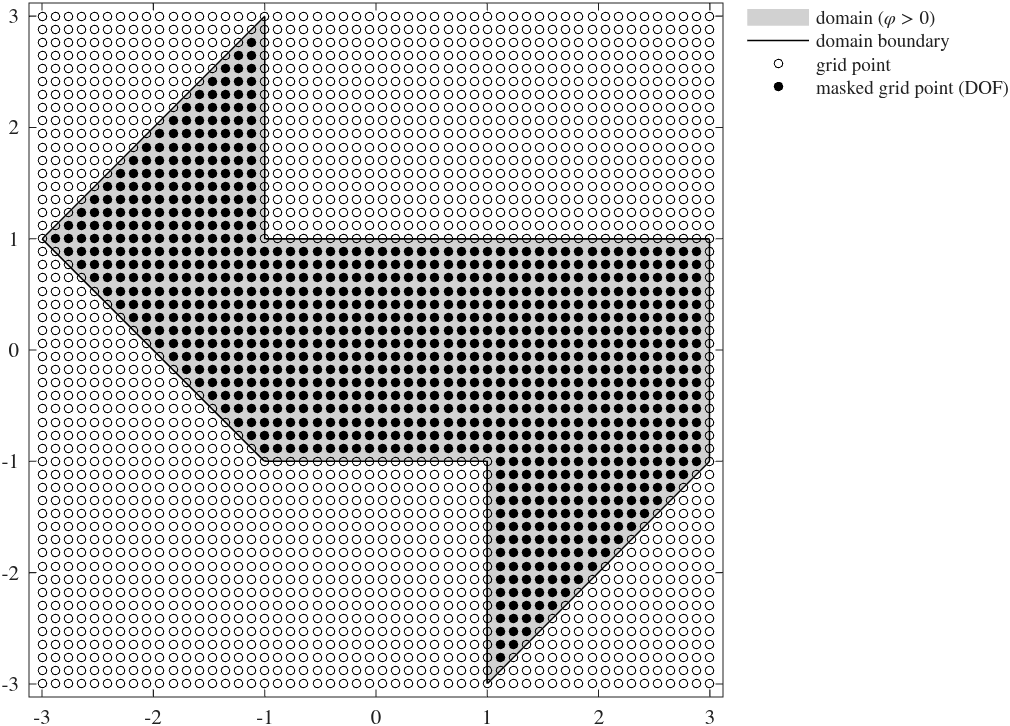
\includegraphics[width=0.4\textwidth]{gww1_grid_M50_dofs936}}
  \qquad
  \subfloat[GWW drum 2, unit building blocks, $M = 50$, DOF $= 936$.]{%
    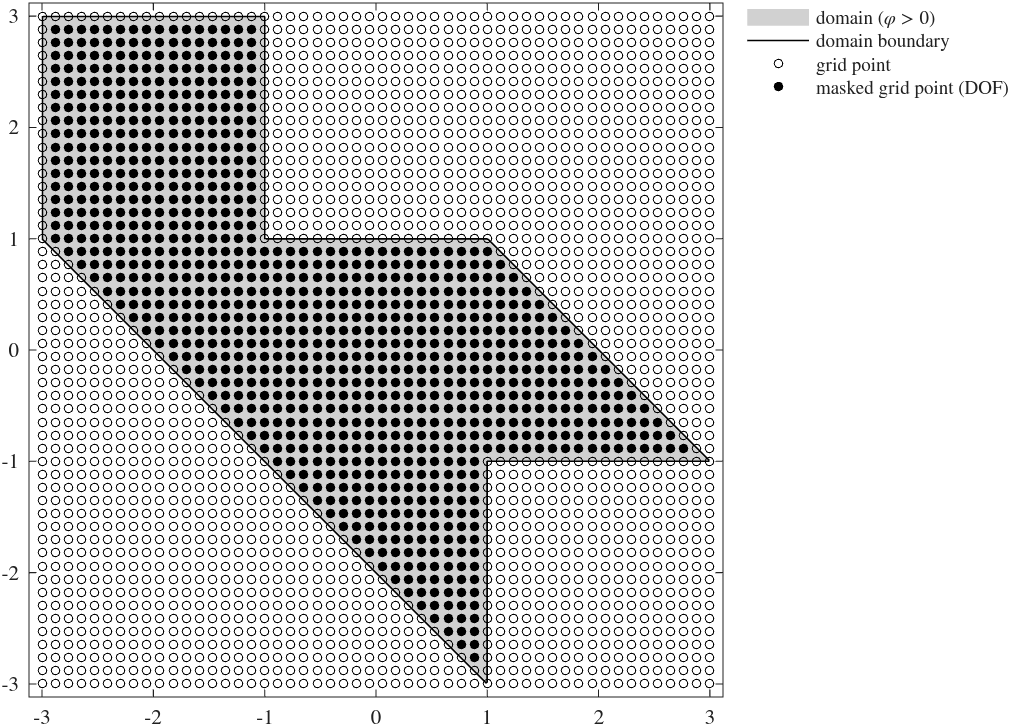
\includegraphics[width=0.4\textwidth]{gww2_grid_M50_dofs936}}
  \\
  \subfloat[Letter H, seven unit squares in a $3 \times 3$ square domain, $M = 50$, DOF $= 1888$.]{%
    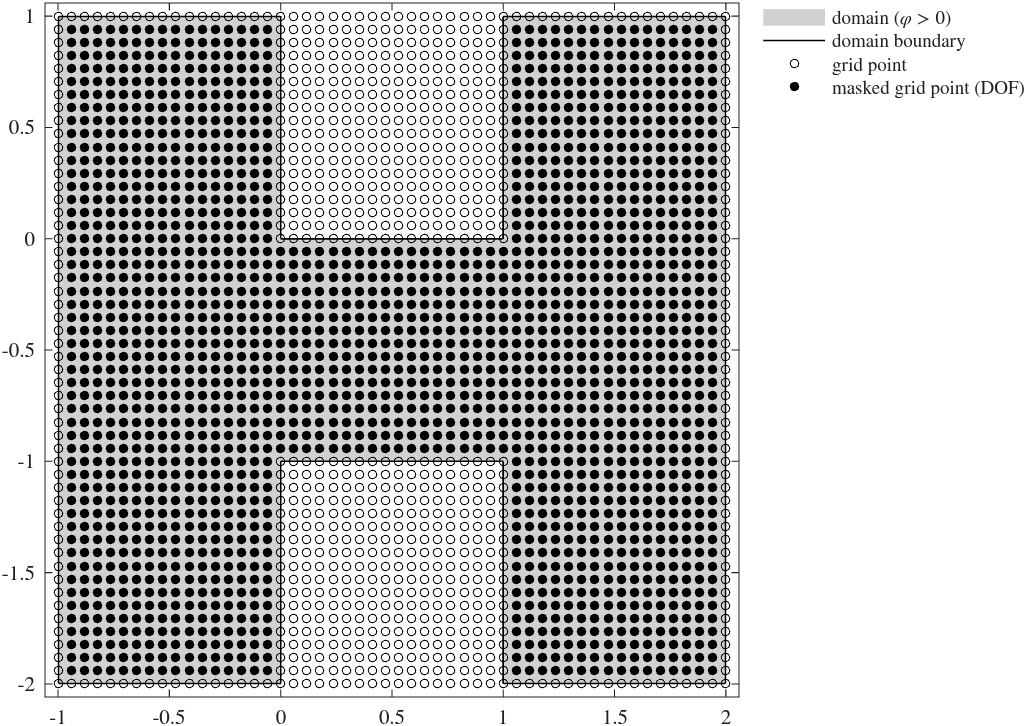
\includegraphics[width=0.4\textwidth]{H_grid_M50_dofs1888}}
  \caption{Domains and DST grids visualisations.}
  \label{fig:domains}
\end{figure}
